\documentclass{article}
\usepackage{graphicx}
\usepackage{caption}
\usepackage{subcaption}
\begin{document}
	
	\begin{figure}
		\centering
		\begin{subfigure}[b]{0.45\textwidth}
			\includegraphics[width=\textwidth]{High/Box34MAR.png}
			\caption{HighMAR}
			\label{fig:HighMAR}
		\end{subfigure}
		~ %add desired spacing between images, e. g. ~, \quad, \qquad, \hfill etc. 
		%(or a blank line to force the subfigure onto a new line)
		\begin{subfigure}[b]{0.45\textwidth}
			\includegraphics[width=\textwidth]{High/Box34MIV.png}
			\caption{HighMIV}
			\label{fig:HighMIV}
		\end{subfigure}
		\newline
		~ %add desired spacing between images, e. g. ~, \quad, \qquad, \hfill etc. 
		%(or a blank line to force the subfigure onto a new line)
		\begin{subfigure}[b]{0.45\textwidth}
			\includegraphics[width=\textwidth]{High/Box34MuOV.png}
			\caption{HighMuOV}
			\label{fig:HighMuOV}
		\end{subfigure}
		\begin{subfigure}[b]{0.45\textwidth}
			\includegraphics[width=\textwidth]{High/Box34MCAR.png}
			\caption{HighMCAR}
			\label{fig:HighMCAR}
		\end{subfigure}
		\caption{High}\label{fig:High}
	\end{figure}
	
	
	\begin{figure}
		\centering
		\begin{subfigure}[b]{0.45\textwidth}
			\includegraphics[width=\textwidth]{Low/Box34MAR.png}
			\caption{LowMAR}
			\label{fig:LowMAR}
		\end{subfigure}
		~ %add desired spacing between images, e. g. ~, \quad, \qquad, \hfill etc. 
		%(or a blank line to force the subfigure onto a new line)
		\begin{subfigure}[b]{0.45\textwidth}
			\includegraphics[width=\textwidth]{Low/Box34MIV.png}
			\caption{LowMIV}
			\label{fig:LowMIV}
		\end{subfigure}
		\newline
		~ %add desired spacing between images, e. g. ~, \quad, \qquad, \hfill etc. 
		%(or a blank line to force the subfigure onto a new line)
		\begin{subfigure}[b]{0.45\textwidth}
			\includegraphics[width=\textwidth]{Low/Box34MuOV.png}
			\caption{LowMuOV}
			\label{fig:LowMuOV}
		\end{subfigure}
		\begin{subfigure}[b]{0.45\textwidth}
			\includegraphics[width=\textwidth]{Low/Box34MCAR.png}
			\caption{LowMCAR}
			\label{fig:LowMCAR}
		\end{subfigure}
		\caption{Low}\label{fig:Low}
	\end{figure}
	
		\clearpage
	


		
		\begin{figure}
			\centering
			\begin{subfigure}[b]{0.45\textwidth}
				\includegraphics[width=\textwidth]{High/Box43MAR.png}
				\caption{HighMAR}
				\label{fig:HighMAR}
			\end{subfigure}
			~ %add desired spacing between images, e. g. ~, \quad, \qquad, \hfill etc. 
			%(or a blank line to force the subfigure onto a new line)
			\begin{subfigure}[b]{0.45\textwidth}
				\includegraphics[width=\textwidth]{High/Box43MIV.png}
				\caption{HighMIV}
				\label{fig:HighMIV}
			\end{subfigure}
			\newline
			~ %add desired spacing between images, e. g. ~, \quad, \qquad, \hfill etc. 
			%(or a blank line to force the subfigure onto a new line)
			\begin{subfigure}[b]{0.45\textwidth}
				\includegraphics[width=\textwidth]{High/Box43MuOV.png}
				\caption{HighMuOV}
				\label{fig:HighMuOV}
			\end{subfigure}
			\begin{subfigure}[b]{0.45\textwidth}
				\includegraphics[width=\textwidth]{High/Box43MCAR.png}
				\caption{HighMCAR}
				\label{fig:HighMCAR}
			\end{subfigure}
			\caption{High}\label{fig:High}
		\end{figure}
		
		\begin{figure}
			\centering
			\begin{subfigure}[b]{0.45\textwidth}
				\includegraphics[width=\textwidth]{Low/Box43MAR.png}
				\caption{LowMAR}
				\label{fig:LowMAR}
			\end{subfigure}
			~ %add desired spacing between images, e. g. ~, \quad, \qquad, \hfill etc. 
			%(or a blank line to force the subfigure onto a new line)
			\begin{subfigure}[b]{0.45\textwidth}
				\includegraphics[width=\textwidth]{Low/Box43MIV.png}
				\caption{LowMIV}
				\label{fig:LowMIV}
			\end{subfigure}
			\newline
			~ %add desired spacing between images, e. g. ~, \quad, \qquad, \hfill etc. 
			%(or a blank line to force the subfigure onto a new line)
			\begin{subfigure}[b]{0.45\textwidth}
				\includegraphics[width=\textwidth]{Low/Box43MuOV.png}
				\caption{LowMuOV}
				\label{fig:LowMuOV}
			\end{subfigure}
			\begin{subfigure}[b]{0.45\textwidth}
				\includegraphics[width=\textwidth]{Low/Box43MCAR.png}
				\caption{LowMCAR}
				\label{fig:LowMCAR}
			\end{subfigure}
			\caption{Low}\label{fig:Low}
		\end{figure}
		
		\clearpage
		
	\begin{figure}
		\centering
		\begin{subfigure}[b]{0.45\textwidth}
			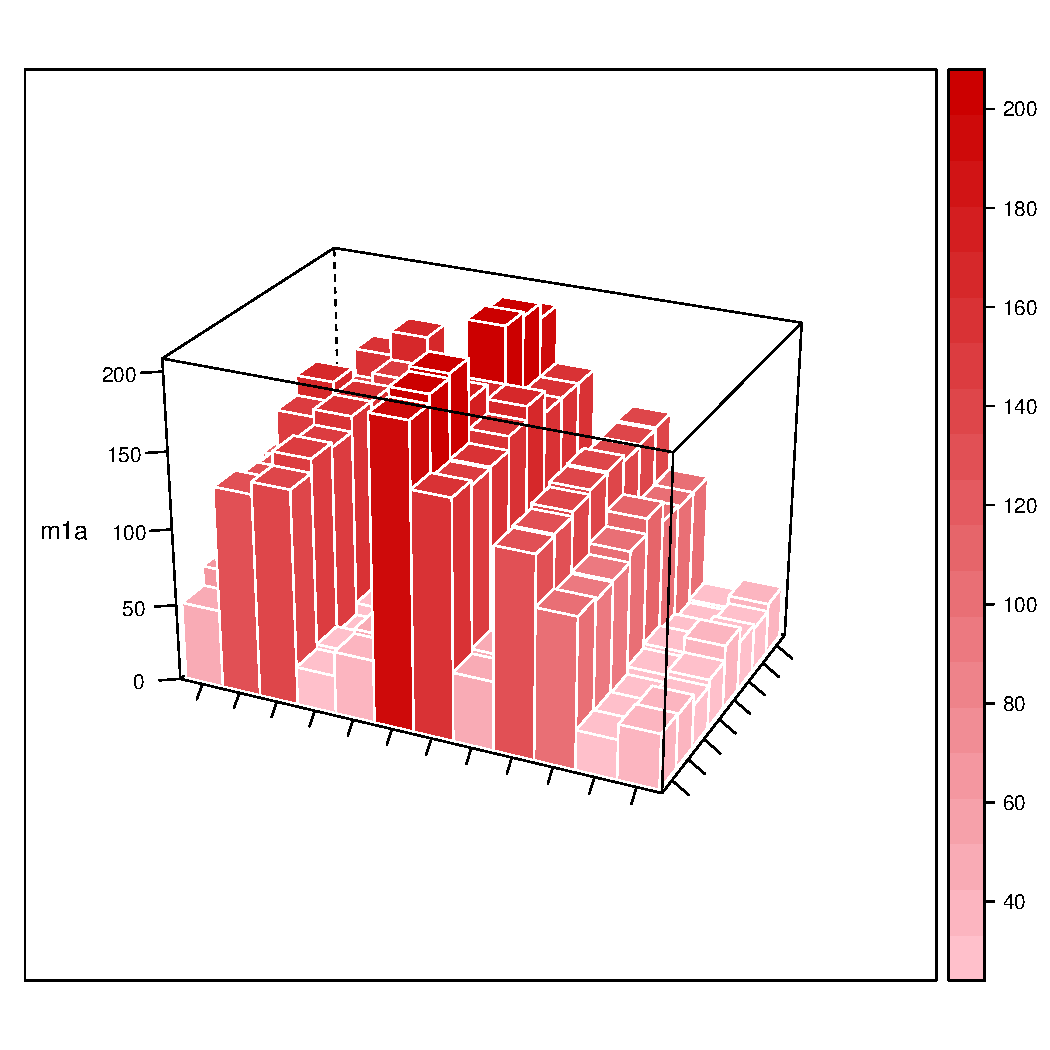
\includegraphics[width=\textwidth]{Low/MAR.pdf}
			\caption{LowMAR}
			\label{fig:LowMAR}
		\end{subfigure}
		~ %add desired spacing between images, e. g. ~, \quad, \qquad, \hfill etc. 
		%(or a blank line to force the subfigure onto a new line)
		\begin{subfigure}[b]{0.45\textwidth}
			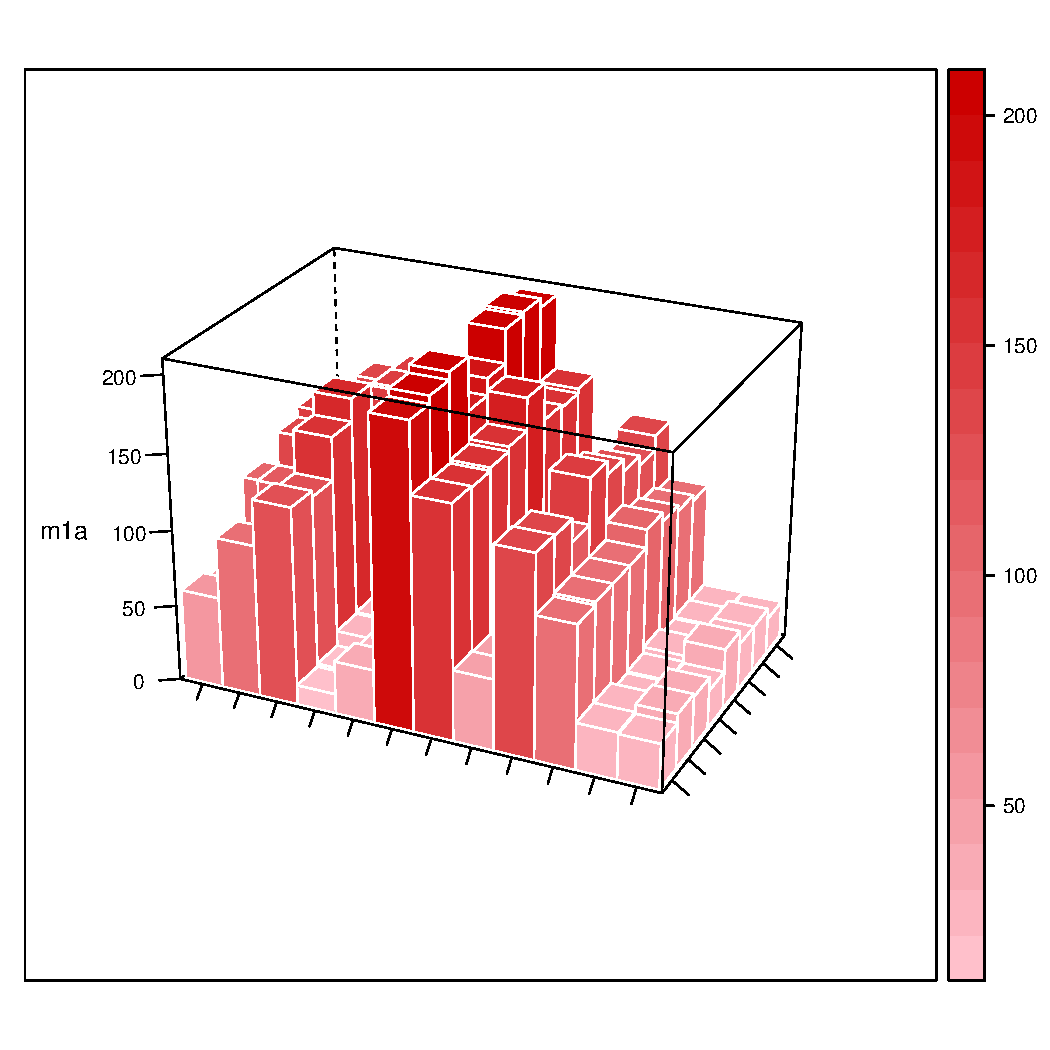
\includegraphics[width=\textwidth]{Low/MIV.pdf}
			\caption{LowMIV}
			\label{fig:LowMIV}
		\end{subfigure}
		\newline
		~ %add desired spacing between images, e. g. ~, \quad, \qquad, \hfill etc. 
		%(or a blank line to force the subfigure onto a new line)
		\begin{subfigure}[b]{0.45\textwidth}
			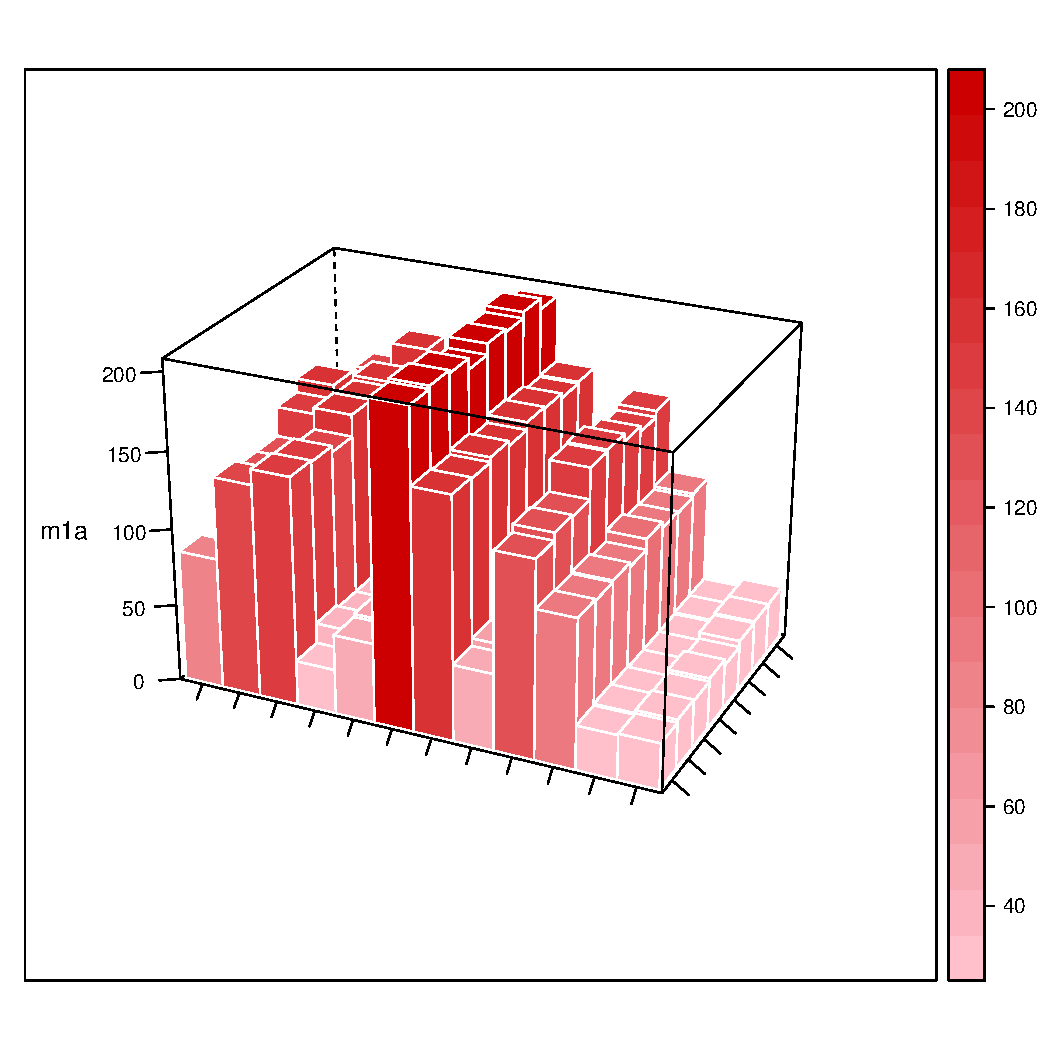
\includegraphics[width=\textwidth]{Low/MuOV.pdf}
			\caption{LowMuOV}
			\label{fig:LowMuOV}
		\end{subfigure}
		\begin{subfigure}[b]{0.45\textwidth}
			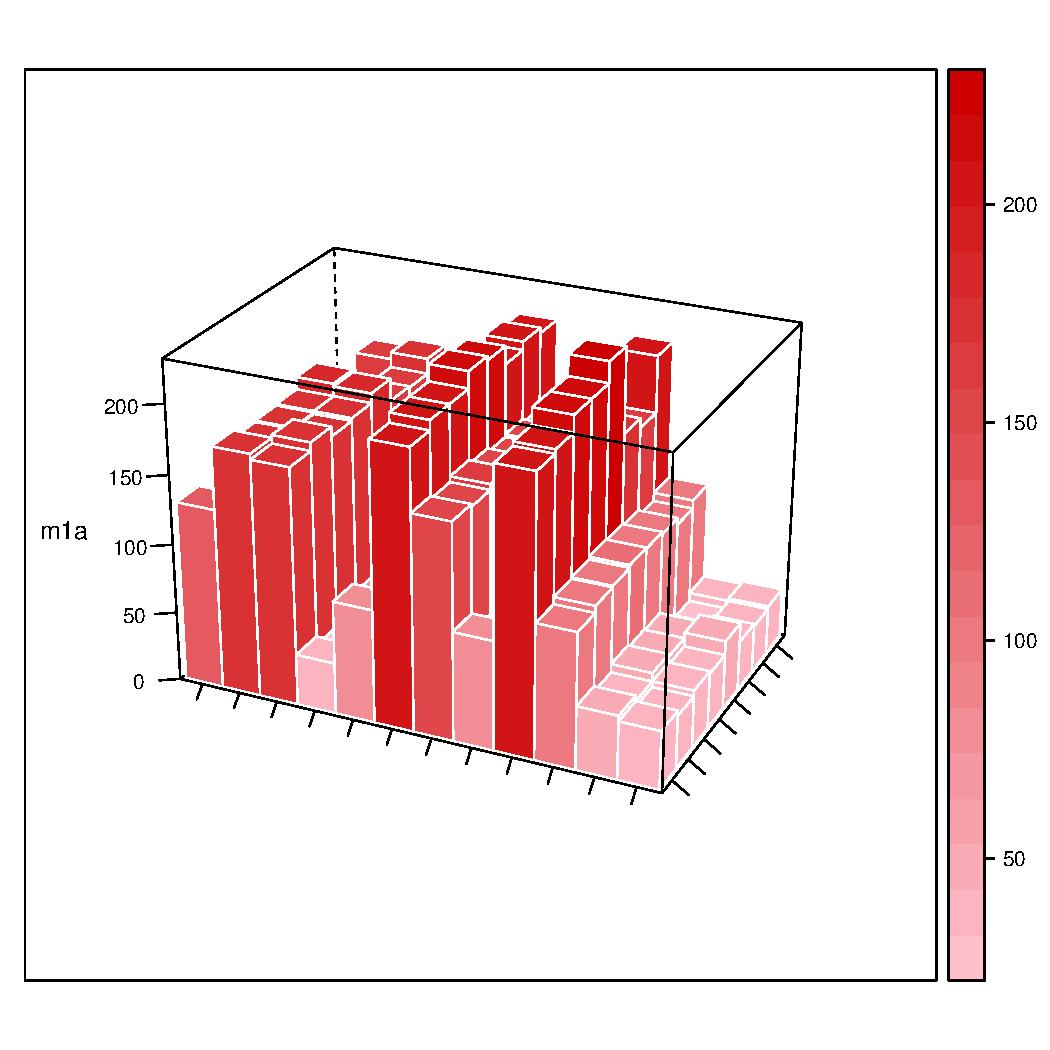
\includegraphics[width=\textwidth]{Low/MCAR.pdf}
			\caption{LowMCAR}
			\label{fig:LowMCAR}
		\end{subfigure}
		\caption{Low}\label{fig:Low}
	\end{figure}
	
			\clearpage
			
					\begin{figure}
						\centering
						\begin{subfigure}[b]{0.45\textwidth}
							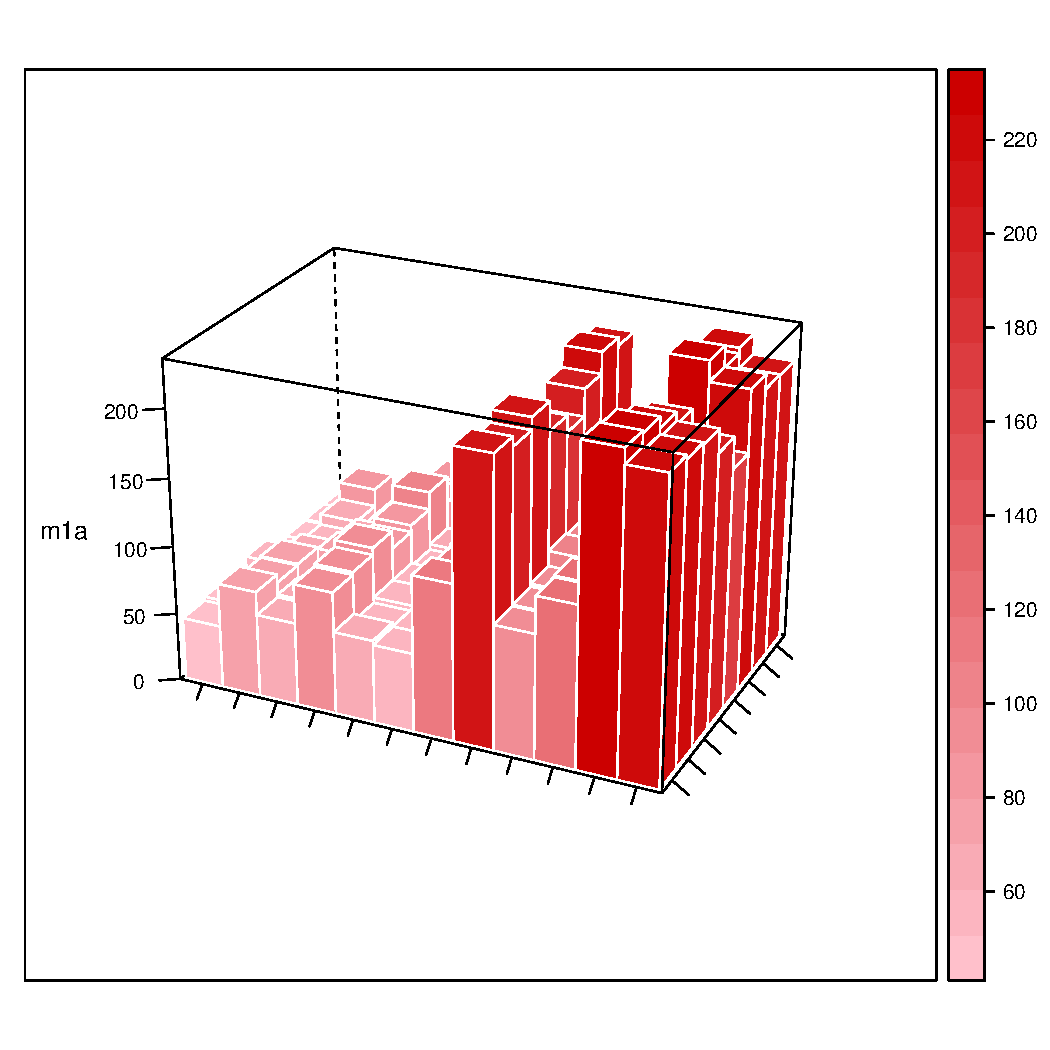
\includegraphics[width=\textwidth]{High/MAR.pdf}
							\caption{HighMAR}
							\label{fig:HighMAR}
						\end{subfigure}
						~ %add desired spacing between images, e. g. ~, \quad, \qquad, \hfill etc. 
						%(or a blank line to force the subfigure onto a new line)
						\begin{subfigure}[b]{0.45\textwidth}
							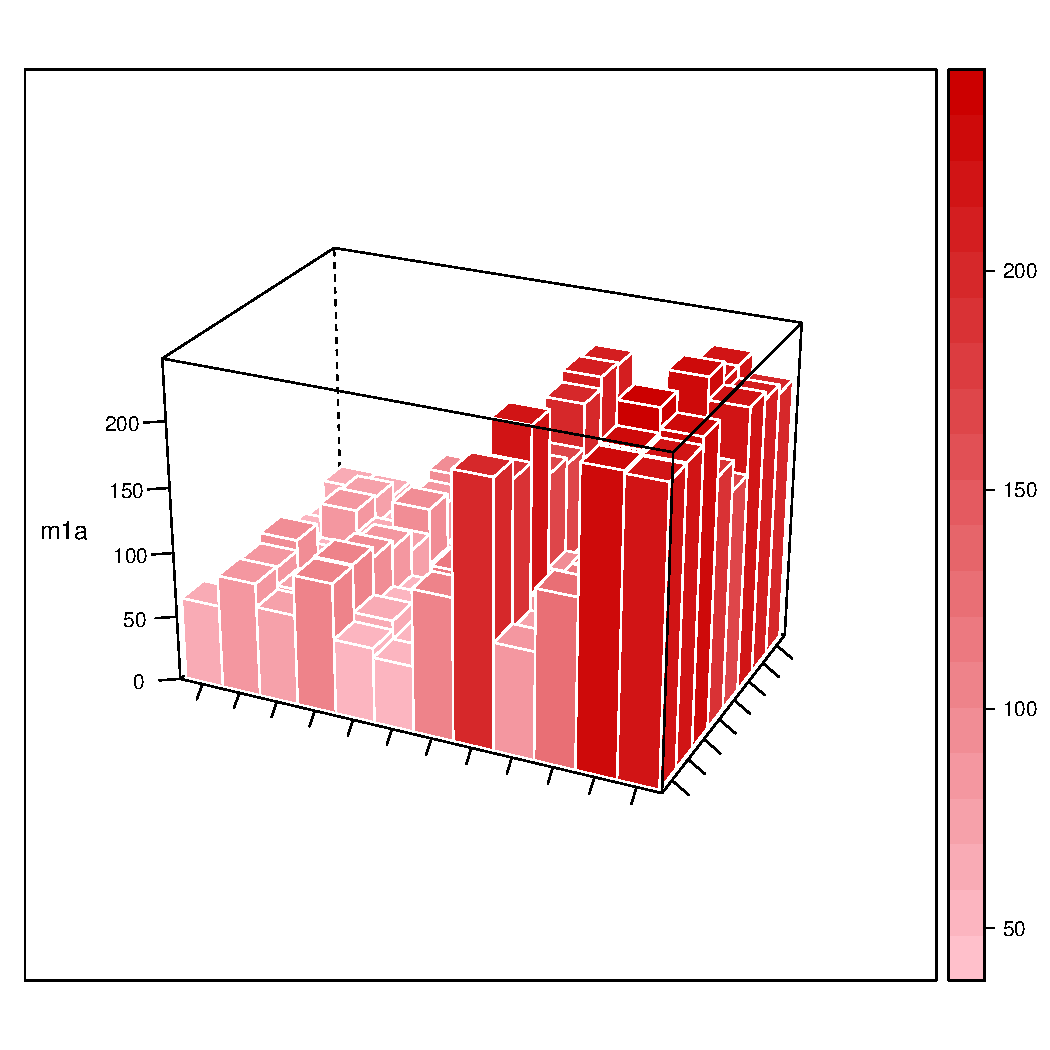
\includegraphics[width=\textwidth]{High/MIV.pdf}
							\caption{HighMIV}
							\label{fig:HighMIV}
						\end{subfigure}
						\newline
						~ %add desired spacing between images, e. g. ~, \quad, \qquad, \hfill etc. 
						%(or a blank line to force the subfigure onto a new line)
						\begin{subfigure}[b]{0.45\textwidth}
							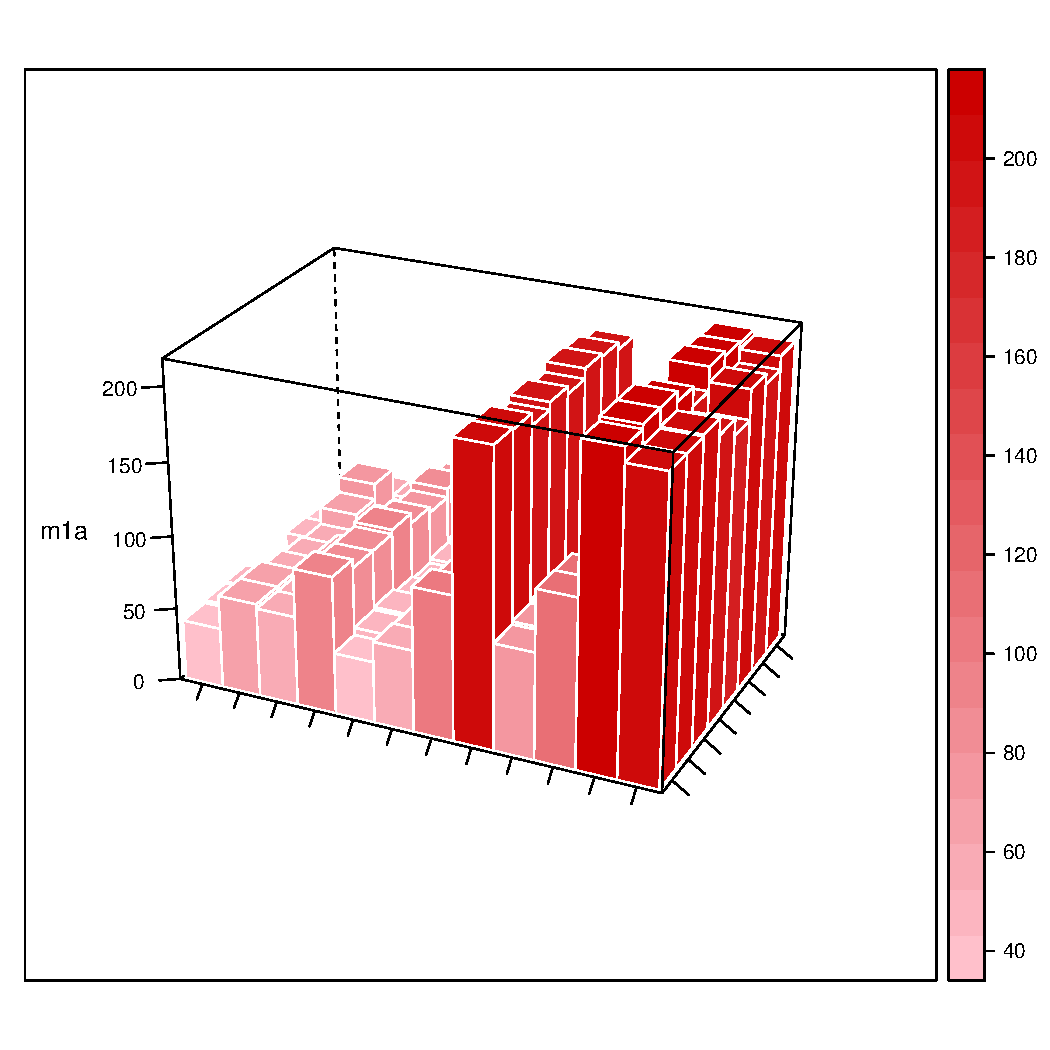
\includegraphics[width=\textwidth]{High/MuOV.pdf}
							\caption{HighMuOV}
							\label{fig:HighMuOV}
						\end{subfigure}
						\begin{subfigure}[b]{0.45\textwidth}
							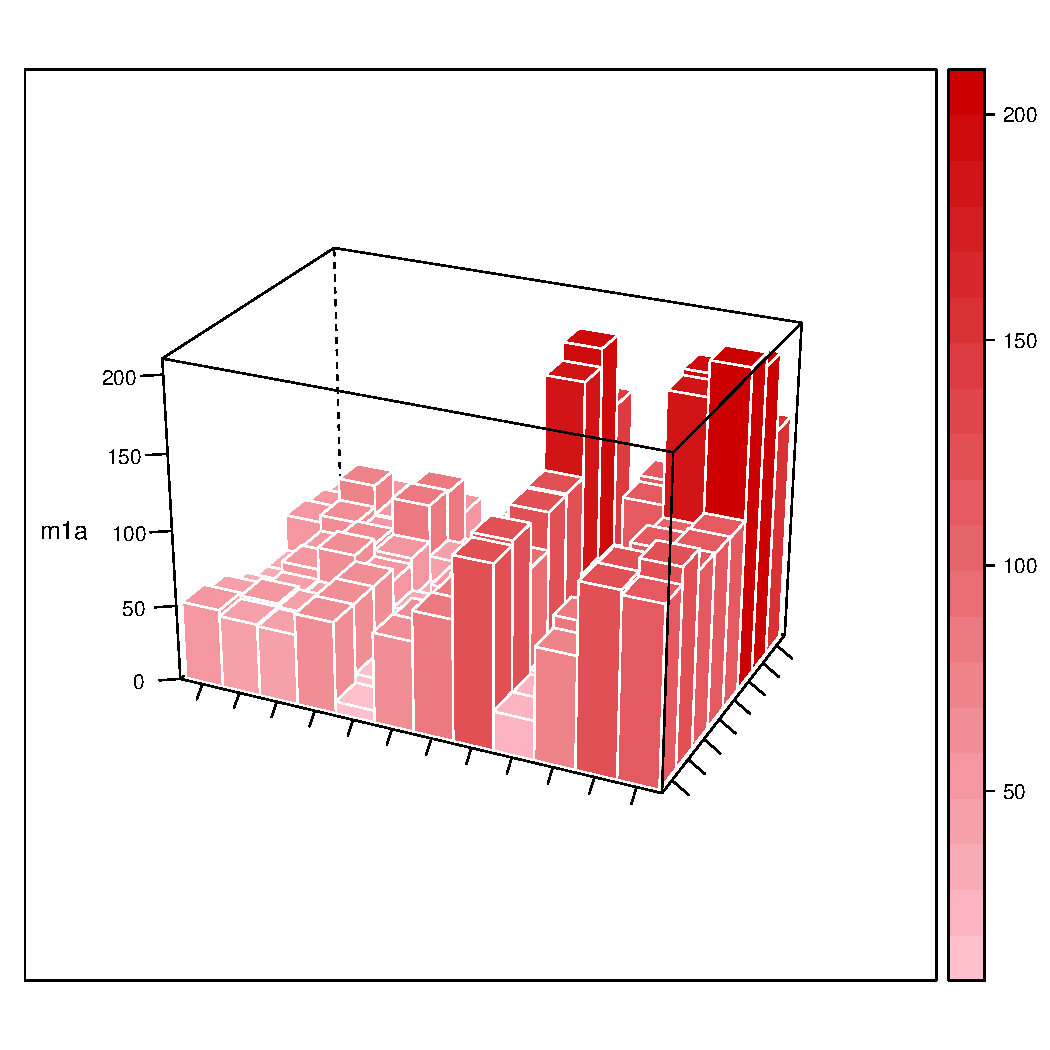
\includegraphics[width=\textwidth]{High/MCAR.pdf}
							\caption{HighMCAR}
							\label{fig:HighMCAR}
						\end{subfigure}
						\caption{High}\label{fig:High}
					\end{figure}
					
					\clearpage
		
			Conclusions1:
			
			\begin{enumerate}
				\item MCAR has more dependence to imputation methods.  
				\item MAR and MuOV are very similar, because even though the algorithm does not contemplate any causative variable, these could be found due to chance, so, practically in some cases it could have the same pattern.
			\end{enumerate}
			
			Conclusions2:
			
			\begin{enumerate}
				\item Differences are less significative.
				\item Even means are almost equal, iterpolation and lvcf offer worse high values, which means that they obtain the worst accuracies. This may be due to the fact that these IM were mainly developed to be used in TS. It makes no sense that one individual's MV is dependent on the previous or posterior individuals' value.
				\item The first three simple methods offer very good results in 3/4 MDT.
				\item When the information about variables is even, complex methods arise.
			\end{enumerate}
			
Seen this, maybe the detect MDType strategy should change to a softer approach, in which the main focus is not to be able to classify the 4 types, but to look for patterns, since MIV, MAR and MuOV have them (stronger or weaker) and MCAR doesn't.
			
			
	
\end{document}